\begingroup
	\usetikzlibrary{calc}
	\pgfdeclarelayer{dibujo}
	\pgfsetlayers{dibujo, main}
	\tikzstyle{zero}=[circle,draw=black,fill=gray,inner sep=0pt,minimum size=2.5mm]
	\tikzstyle{one}=[circle,draw=black,fill=black,inner sep=0pt,minimum size=2.5mm]
	\tikzstyle{two}=[circle,draw=black,fill=white,inner sep=0pt,minimum size=2.5mm]
	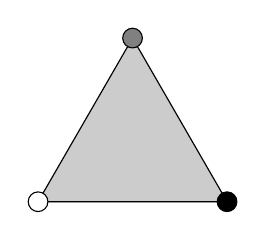
\begin{tikzpicture}
		\begin{pgfonlayer}{dibujo}
			\filldraw [fill=black,opacity=0.2] (0,0)--(2.4,0)--($ (0,0) ! 1 ! 60:(2.4,0) $)--(0,0);
			\draw (0,0)--(2.4,0)--($ (0,0) ! 1 ! 60:(2.4,0) $)--(0,0);
		\end{pgfonlayer}
		\node[two] (o) at (0,0) {};
		\node[white] (op) at (2.4,0) [one] {};
		\node[zero] (opp) at ($ (o) ! 1 ! 60:(op) $) {};	
	\end{tikzpicture}
%	\label{fig:2_simplex}
\endgroup